
\chapter{Общие сведения}
\label{chapter1}

В течение многих десятилетий основой испанской энергетики был уголь, но доля его в производстве первичной энергии постоянно сокращалась (из-за его плохого качества и малой производительности угольных шахт), и одновременно росла доля гидроэнергии и нефти. Испания своей нефти почти не имеет, поэтому чрезвычайно увеличилась зависимость энергетики Испании от крупнейших нефтяных монополий мира, и в 1990-х годах за счет этого источника обеспечивалось 80\% энергопотребления. Хотя с начала 1960-х годов в Испании были обнаружены несколько месторождений нефти (в 1964 была найдена нефть в 65 км к северу от Бургоса, а в начале 1970-х годов – близ Ампосты в дельте Эбро), использование отечественных источников энергии не поощряется.

В 1992 в общем балансе производства электроэнергии почти половина приходилась на долю местного угля и импортной нефти, 36\% – на долю ядерного топлива и 13\% – на долю гидроэнергии. Из-за низкого энергетического потенциала рек Испании роль гидроэнергетики сильно сократилась (в 1977 она давала 40\% выработанной электроэнергии). Благодаря наличию больших запасов урана был разработан план развития атомной энергетики. Первая АЭС была запущена в 1969, однако в 1983 по экологическим соображениям был введен запрет на строительство новых АЭС. Стоимость энергоносителей начала расти, наступило время обдумать сложившуюся ситуацию. Испания приняла решение пойти на развитие энергетики, основанной на собственных энергоресурсах. Больше всего в Испании солнечной энергии. Испания горная страна, поэтому энергии ветра так же немало. Оказалось, что для Испании ветер более доступен, а Солнце более перспективно. Оно и понятно. Общий энергетический потенциал ветра на Земле в 160 раз превышает совокупную мощность всех электростанций, а солнечного излучения, падающего на Землю более, чем в 2000 раз! Но ветер сегодня дает более дешевую энергию.

Сегодня основным критерием политики Испании является самодостаточность в производстве электроэнергии.
• Испания имеет восемь ядерных реакторов, генерирующих 16\% электроэнергии страны.
• С точки зрения общей генерирующей мощности, сектор возобновляемых источников энергии Испании уступает только США и Германии - 17\% производства электроэнергии
• Оставшиеся 31\% и 9\% в энергетическом балансе приходятся на газ и уголь соответственно.

Энергия ветра является третьим источником электроэнергии в Испании после газа и атомной энергии. В 2011 году энергия ветра покрывала 15\% электрического спроса в стране. Испания вторая по величине суммарной установленной мощности ветровой энергетики в Европе, и четвертая в мире после США, Германии и Китая.
В апреле 2012 г. в ветровой энергетике Испании был поставлен рекорд: было произведено более 5000 ГВт-ч в месяц!

Испания по существу отделена от энергосистемы ЕС, мало того что она полностью обеспечивает энергией себя, также продает небольшую часть Франции.

В диаграмме  можно увидеть структуру электрогенерации в Испании за январь-август 2016

\begin{figure}[h]
	\begin{center}
		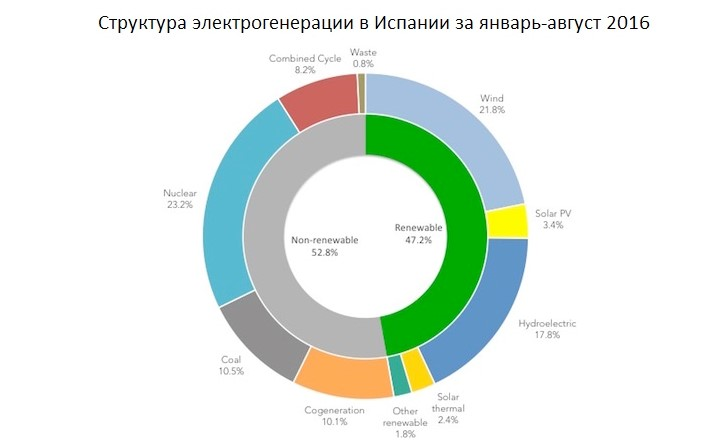
\includegraphics[width=.5\columnwidth]{./img/Spain-energy.jpg}
	\end{center}
	\caption{Структуру электрогенерации в Испании за январь-август 2016}
	\label{pic:struct_energy}
\end{figure}








